\documentclass{beamer}
\usepackage{graphicx}
\usepackage{paralist}
\usepackage{outlines}

\title{Healing Brushes}
\author{Mendocino College - Digital Image Manipulation with Photoshop}
\titlegraphic{\vspace{-10mm}
\includegraphics[width = .9\textwidth]{images/photoshop.jpg}} 
\date{\vspace{-5em}} 


\mode <presentation>
\usetheme{Warsaw}
\usecolortheme{default}

\setbeamerfont{footline}{size=\fontsize{5}{8}\selectfont}

\definecolor{darkred}{rgb}{20,0,0}
\definecolor{darkgreen}{RGB}{40,110,20}
\definecolor{darkpurple}{RGB}{30,0,30}
\definecolor{chardonnay}{RGB}{255, 255, 204}

\setbeamercolor*{palette primary}{fg=white, bg=darkgreen}


\begin{document}
	{
		\setbeamertemplate{footline}{} 
		\setbeamertemplate{headline}{} 
		\begin{frame}
			\vspace{-35pt}
			\maketitle
		\end{frame}
	}
		
		
\section{Healing Brush}

\subsection{Healing Brush}		

	\begin{frame}
		\frametitle{Healing Brush}
		\begin{outline}
			\1 
		\end{outline}
	\end{frame}

\subsection{Example}		
	\begin{frame}
		\frametitle{Healing Brush Example}
		\begin{center}
			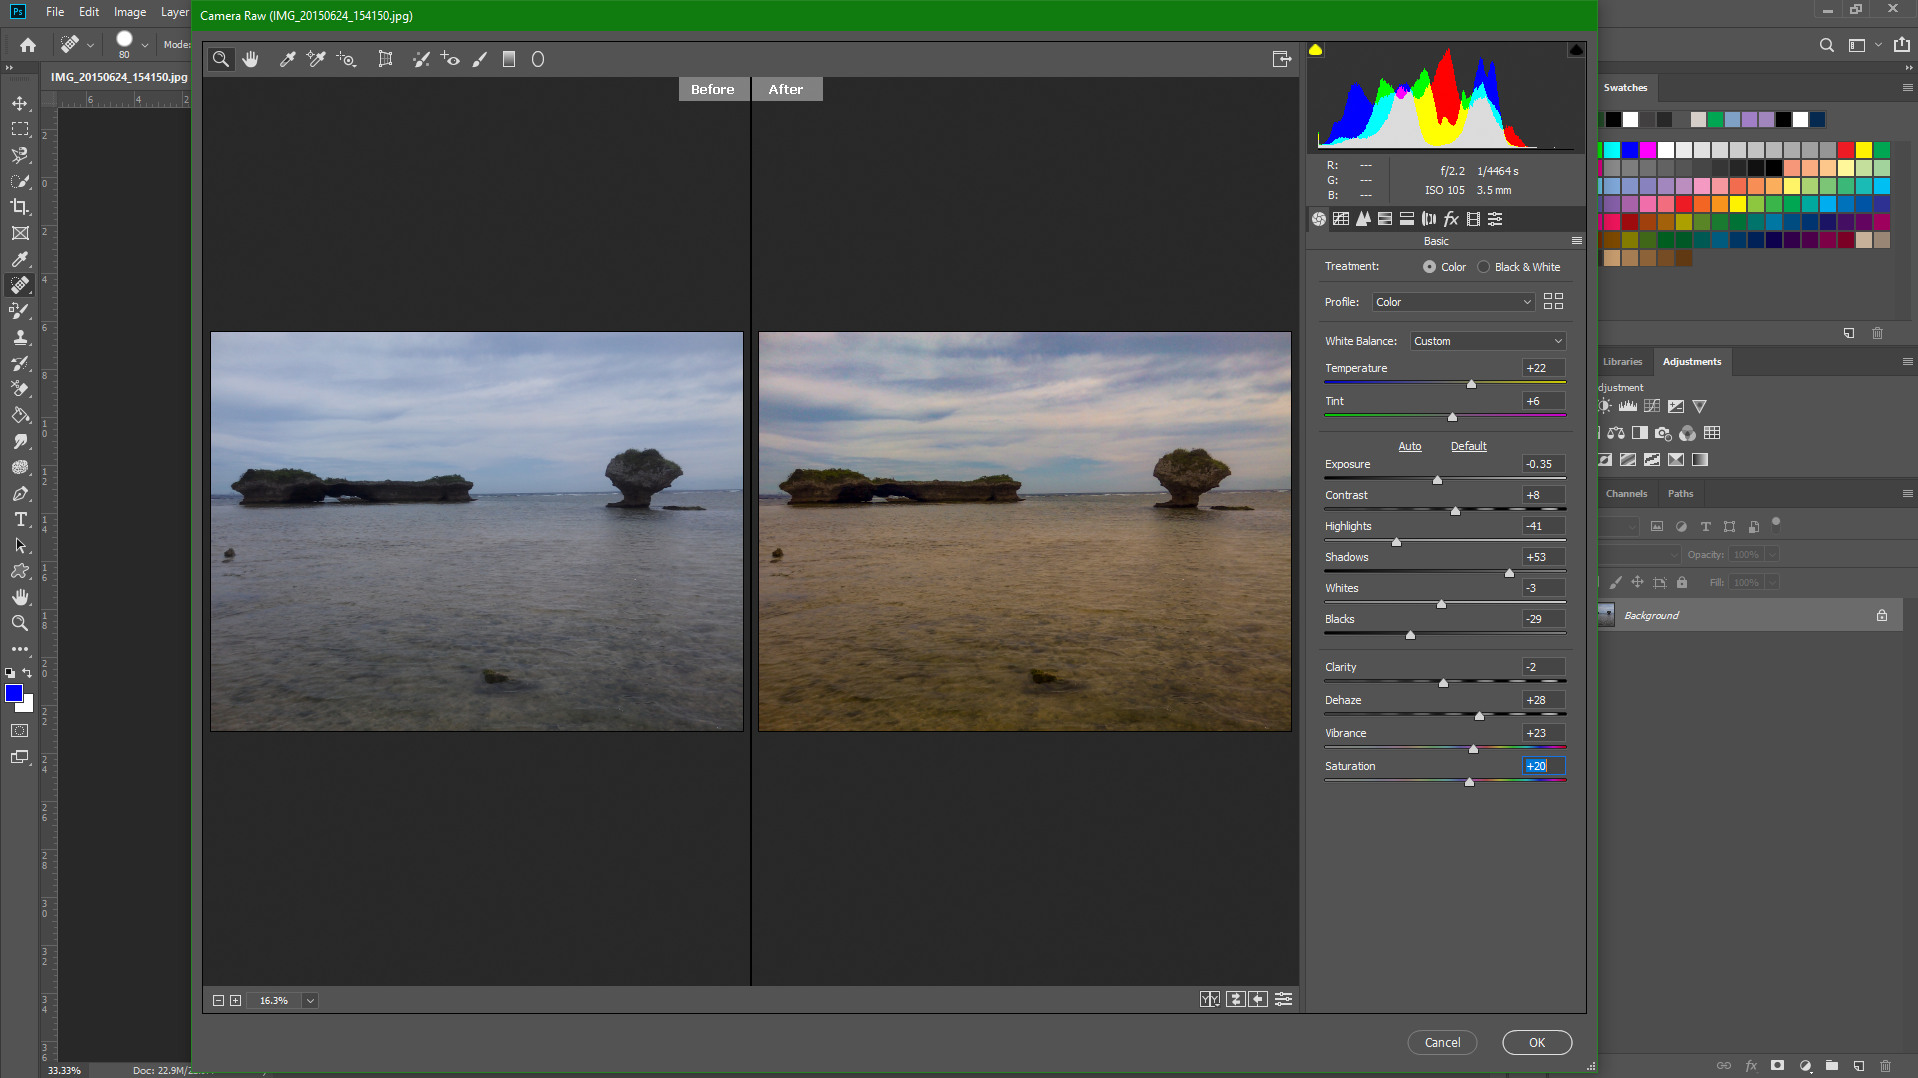
\includegraphics[width=1.10\textwidth]{images/Camera raw filter example.png}
		\end{center}
	\end{frame}

\subsection{Options}		
	\begin{frame}
		\frametitle{Healing Brush Options}
		\begin{outline}
			\1 
		\end{outline}
	\end{frame}

\subsection{Resources}		
	\begin{frame}
		\frametitle{Additional Resources for the Healing Brush}
		\begin{outline}
			\1 
		\end{outline}
	\end{frame}


\section{Spot Healing Brush}

\subsection{Spot Healing Brush}		

\begin{frame}
	\frametitle{Spot Healing Brush}
	\begin{outline}
		\1 
	\end{outline}
\end{frame}

\subsection{Example}		
\begin{frame}
	\frametitle{Spot Healing Brush Example}
	\begin{center}
		\includegraphics[width=1.0\textwidth]{images/Spot Healing Brush example.png}
	\end{center}
\end{frame}

\subsection{Options}		
\begin{frame}
	\frametitle{Spot Healing Brush Options}
	\begin{outline}
		\1 
	\end{outline}
\end{frame}

\subsection{Resources}		
\begin{frame}
	\frametitle{Additional Resources for the Spot Healing Brush}
	\begin{outline}
		\1 
		\2 
		\2
	\end{outline}
\end{frame}
	
\end{document}